%%%%%%%%%%%%%%%%%%%%%%%%%%%%%%%%%%%%%%%%%
%
% (c) 2022 by Jennifer Laaser
%
% This work is licensed under the Creative Commons Attribution-NonCommercial-ShareAlike 4.0 International License. To view a copy of this license, visit http://creativecommons.org/licenses/by-nc-sa/4.0/ or send a letter to Creative Commons, PO Box 1866, Mountain View, CA 94042, USA.
%
% The current source for these materials is accessible on Github: https://github.com/jlaaser/pogil-polymers
%
%%%%%%%%%%%%%%%%%%%%%%%%%%%%%%%%%%%%%%%%%

\renewcommand{\figpath}{content/polymchem/freeradical/FRPthermo/figs}
\renewcommand{\labelbase}{FRPthermo}

\begin{activity}{Thermodynamics of Free-Radical Polymerization}

\begin{instructornotes}
	This activity introduces students to concepts related to the thermodynamics of free-radical polymerization.
	
	After completing this activity, students will be able to:
	\begin{enumerate}
		\item Identify the signs of the enthalpy and entropy changes during a propagation step and explain why propagation is considered an \emph{enthalpically-driven} process
		\item Explain why there is a certain temperature above which propagation is expected to stop, and calculate this temperature from relevant thermodynamic quantities
		\item Describe how the reaction rates in a free-radical polymerization are expected to change as the reaction proceeds, and explain how this leads to autoacceleration in polymerizations carried out at high monomer concentrations
	\end{enumerate}
	
	\subsection*{Activity summary:}
	\begin{itemize}
		\item \textbf{Activity type:} Learning Cycle
		\item \textbf{Content goals:} See above
		\item \textbf{Process goals:} %https://pogil.org/uploads/attachments/cj54b5yts006cklx4hh758htf-process-skills-official-pogil-list-2015-original.pdf
			\begin{itemize}
				\item Interpreting reaction schemes and equations
				\item Manipulating equations to derive a result
				\item Written and oral communication of reasoning
			\end{itemize}
		\item \textbf{Duration:} 45 min
		\item \textbf{Instructor preparation required:} none beyond knowledge of relevant content
		\item \textbf{Related textbook chapters:}
			\begin{itemize}
				\item \emph{Polymer Chemistry} (Hiemenz \& Lodge), 2nd ed.: section 4.7
				\item \emph{Introduction to Polymers} (Young \& Lovell), 3rd ed.: section 4.3.10.1
			\end{itemize}
		%\item \textbf{Facilitation notes:}
		%	\begin{itemize}
		%		\item \dots
		%	\end{itemize}
	\end{itemize}
	
\end{instructornotes}


\begin{model}[Thermodynamics of Propagation]
	\label{\labelbase:mdl:propthermo}

	The propagation step of a free-radical polymerization is shown below:
	
	\centerline{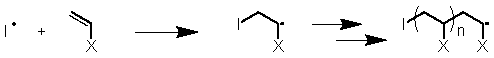
\includegraphics[width=0.8\textwidth]{\figpath/Model1-prop}}
	
	%In this model, we will investigate the thermodynamics of this propagation step.
	
\end{model}


\begin{ctqs}

	\question First, let's think about the enthalpy of the radical center. \label{\labelbase:ctq:radicalenthalpy}
	
		\begin{enumerate}
		
			\item Does the ``type'' of radical change in this propagation step?
				
				\begin{solution}[0.5in]{}
					No, the radical is (in this case) a secondary radical with identical neighboring substituents both before and after addition of the monomer.
				\end{solution}
			
			\item Based on your answer to part (a), do you expect the radical center to contribute significantly to the enthalpy of the reaction?  Briefly explain your group's reasoning.
				
				\begin{solution}[1in]{}
					No, because the radical's structure doesn't change, the enthalpy of the radical center should be essentially the same before and after monomer addition, so it will not contribute significantly to the enthalpy of the reaction.
				\end{solution}
			
		\end{enumerate}
		
	\question Second, let's think about the enthalpy of the bonds. \label{\labelbase:ctq:bondenthalpy}
	
		\begin{enumerate}
			\item How does the number of C-C single bonds change in this propagation step?
			
				\emph{Note: for the purposes of this question, do not count the C=C bond in the monomer as ``containing'' a single bond - before it is polymerized, it gets counted as a double bond only!}
				
				\begin{solution}[1in]{}
					Increases by 2
				\end{solution}
			
			\item How does the number of C=C double bonds change in this propagation step?
				
				\begin{solution}[0.75in]{}
					Decreases by 1
				\end{solution}
			
			\item Typical enthalpies of formation for C-C and C=C bonds are summarized below:
				
				\begin{center}
					\renewcommand{\arraystretch}{1.5}
					\begin{tabular}{c c}
						\hline
						Bond Type & $\Delta H$ (kJ/mol) \\\hline
						C-C	&	-350 \\
						C=C &	-610 \\\hline
					\end{tabular}
				\end{center}
				
				Based on this information, calculate the enthalpy change for the propagation reaction shown in Model \ref{\labelbase:mdl:propthermo}.
				
				\begin{solution}[1.25in]{}
					\begin{align*}
						\Delta H_{rxn} &= 2\Delta H(\text{C-C}) - \Delta H (\text{C=C})\\
							&= 2(-350\text{ kJ/mol}) - (-610\text{ kJ/mol})\\
							&= -90\text{ kJ/mol}
					\end{align*}
				\end{solution}
		\end{enumerate}
		
	\question Based on your answers to CTQs \ref{\labelbase:ctq:radicalenthalpy} and \ref{\labelbase:ctq:bondenthalpy}, do you expect the propagation step to be exothermic (releases heat) or endothermic (requires heat input)?
	
		\emph{Hint: remember that negative values of $\Delta H$ correspond to exothermic reactions.}
				
				\begin{solution}[0.75in]{}
					$\Delta H$ is negative, so the propagation step is exothermic
				\end{solution}
		
	\question Next, let's consider how the entropy changes in this propagation step.
	
		\begin{enumerate}
			
			\item How does the total number of molecules present in the reaction mixture change in this reaction?
				
				\begin{solution}[0.5in]{}
					Decreases by 1 (monomer becomes part of the polymer chain)
				\end{solution}
			
			\item Does the translational freedom of the monomer increase or decrease as it attaches to the polymer chain?
				
				\begin{solution}[0.5in]{}
					The translational freedom of the monomer decreases because it is now restricted to move only where the polymer chain goes
				\end{solution}
			
			\item Based on your answers to the previous two questions, do you expect the overall entropy of the system to increase or decrease in this propagation step?  Briefly explain your group's reasoning.
				
				\begin{solution}[1.25in]{}
					The entropy of the system decreases because the monomer's motion is more restricted once it connects to the polymer chain.  As a result, the total ``number of ways'' that the system can arrange itself decreases, decreasing the entropy.
				\end{solution}
			
		\end{enumerate}
	
	\question Based on your answers, would you characterize the propagation step in free-radical polymerization as an ``enthalpy-driven'' reaction or as an ``entropy-driven'' reaction?  Briefly explain your group's reasoning in 1-2 complete sentences.
	
		\begin{solution}[1.25in]{}
			This reaction is an enthalpy-driven reaction.  Decreases in entropy are generally unfavorable, so it must be the exothermicity of the reaction that helps make it favorable.
			
			Quantitatively, a reaction is favorable when $\Delta G = \Delta H - T\Delta S < 0$.  Here, $\Delta H < 0$ and contributes favorably to making $\Delta G < 0$.  $\Delta S < 0$ means that $-T \Delta S > 0$, so the entropic term does \emph{not} contribute favorably to making $\Delta G < 0$.
		\end{solution}
		
	\question Is there a temperature above which the propagation reaction will no longer be favorable?  Explain your group's reasoning in 1-2 complete sentences.\label{\labelbase:ctq:ceilingconcept}
	
		\begin{solution}[1.25in]{}
			Yes.  Once $T\Delta S$ is greater in magnitude than $\Delta H$, $\Delta G$ will become positive and the reaction will no longer be favorable.
			
			Note that we have not asked students to solve for $T_c$ here because they will come out with $T_c = \Delta H/\Delta S$.  This relationship misses the dependence on monomer concentration, which is explored in more detail in the next model.
		\end{solution}

\end{ctqs}




\begin{model}[Equilibrium of Propagation]
	\label{\labelbase:mdl:propequilib}

	In our discussion of the kinetics of free radical polymerization, we depicted propagation as being a ``one-way street'' - i.e. the reaction arrow only pointed to the right:
	
	\begin{equation*}
		\text{\ce{P_n^.} + M} \xlongrightarrow{} \text{\ce{P_{n+1}^.}}
	\end{equation*}
	
	However, in reality, this reaction can actually go either forward or backward, and it is more appropriate to write it as an equilibrium, as follows:
	
	\begin{equation*}
		\text{\ce{P_n^.} + M} \rightleftharpoons{} \text{\ce{P_{n+1}^.}}
	\end{equation*}
	
	At equilibrium, the concentration of monomer in the reaction mixture will be $[\text{M}]_{eq}$.
	
\end{model}


\begin{ctqs}

	\question Write an appropriate equilibrium constant for this reaction, in terms of [\ce{P_n^.}], [\ce{P_{n+1}^.}], and $[\text{M}]_{eq}$.
				
				\begin{solution}[1in]{}
					\begin{equation*}
						K_{eq} = \frac{[\ce{P_{n+1}^.}]}{[\ce{P_n^.}][\text{M}]_{eq}}
					\end{equation*}
				\end{solution}
	
	\question In most polymerizations, [\ce{P_n^.}]$\approx$[\ce{P_{n+1}^.}].  Use this approximation to rewrite your equilibrium constant from the previous problem as a function of the equilibrium monomer concentration, $[M]_{eq}$, only.
				
				\begin{solution}[0.5in]{}
					\begin{equation*}
						K_{eq}\approx \frac{1}{[\text{M}]_{eq}}
					\end{equation*}
				\end{solution}
	
	\question Recall that a reaction is in equilibrium when $K = e^{-\Delta G^\circ/RT}$.  Use this relationship, and the fact that $\Delta G^\circ = \Delta H^\circ - T\Delta S^\circ$, to write an  expression for the equilibrium monomer concentration in terms of the $\Delta H$ and $\Delta S$ of the propagation reaction. \label{\labelbase:ctq:Meq}
				
				\begin{solution}[1in]{}
					\begin{align*}
						\frac{1}{[\text{M}]_{eq}} &= e^{-\Delta G^\circ/RT} = e^{-(\Delta H^\circ - T\Delta S^\circ)/RT}\\
						[\text{M}]_{eq} &= e^{(\Delta H^\circ - T\Delta S^\circ)/RT}
					\end{align*}
				\end{solution}
	
	\question Suppose you have a polymerization reaction whose equilibrium monomer concentration is $[M]_{eq}$.  
		\begin{enumerate}
			\item If you start a reaction with a concentration of monomer $[\text{M}] < [\text{M}]_{eq}$, will any polymer form?  Why or why not?
				
				\begin{solution}[1in]{}
					By Le Chatelier's principle, if $[\text{M}] < [\text{M}]_{eq}$, it is essentially like starting at equilibrium and removing monomer (a reagent).  This should pull the reaction ``to the left'' and prevent polymer from forming (if some polymer radicals have already formed, this condition would cause depolymerization, not polymerization).
				\end{solution}
				
			\item If you start a reaction with a concentration of monomer $[\text{M}] > [\text{M}]_{eq}$, will any polymer form?  Why or why not?
				
				\begin{solution}[1in]{}
					By Le Chatelier's principle, if $[\text{M}] > [\text{M}]_{eq}$, it is essentially like starting at equilibrium and adding excess monomer (a reagent).  This should push the reaction to the right and drive formation of polymer.
				\end{solution}
				
			\item Once a polymerization reaction consumes enough monomer to reach its equilibrium monomer concentration, will the polymer chains continue to grow?  Explain your group's reasoning in 1-2 complete sentences.
				
				\begin{solution}[1.5in]{}
					No. Once the reaction consumes enough monomer to reach its equilibrium monomer concentration, then there is no driving force to form more polymer.
					
					Note that this does not mean that no propagation steps occur - it just means that depolymerization (reverse of propagation) is happening at exactly the same rate, so there is no \emph{net} consumption of monomer.
				\end{solution}
				
		\end{enumerate}
	
	\question The previous two questions considered how the equilibrium depends on the monomer concentration at a fixed temperature. However, it is also useful to consider how the equilibrium depends on the temperature at a given monomer concentration.
	
		\begin{enumerate}
		
			\item Rearrange your answer to CTQ \ref{\labelbase:ctq:Meq} to solve for the temperature $T_c$ at which the reaction is in equilibrium with a monomer concentration $[\text{M}]_{eq}$.
				
				\begin{solution}[1in]{}
					\begin{align*}
						T_c = \frac{\Delta H^\circ}{\Delta S^\circ + R \ln [\text{M}]_{eq}}
					\end{align*}
				\end{solution}
				
			\item Explain why $T_c$ (which we refer to as the ``ceiling temperature'' of the reaction) can be considered to be the maximum temperature at which polymer will form in a reaction with monomer concentration $[\text{M}]_{eq}$. \emph{Hint: think back to your answer to CTQ \ref{\labelbase:ctq:ceilingconcept}!}.
				
				\begin{solution}[1.5in]{}
					This is the temperature above which $\Delta G > 0$.  When $\Delta G > 0$, the propagation reaction is no longer favorable, and no more polymer will form.
				\end{solution}
				
		\end{enumerate}

\end{ctqs}



\begin{model}[Changes to Reaction Rates During Polymerization]
\label{\labelbase:mdl:rxnrates}

	In our derivation of the kinetics of free radical polymerization, we assumed that the rate constants for each step ($k_d$, $k_p$, and $k_t$) did not change over the course of the reaction.  In real polymerizations, however, this does not always hold true.

\end{model}

\begin{ctqs}

	\question As a polymerization reaction progresses, and more and more and more monomer is converted to polymer, what do you expect to happen to the viscosity of the reaction mixture?  Explain your group's reasoning in 1-2 complete sentences.
	
		\begin{solution}[1.5in]{}
			The reaction mixture should become more viscous.  Generally, polymers and polymer solutions are more viscous than the monomers because they are much larger.		
		\end{solution}
		
	\question As the viscosity of the reaction mixture changes, do you expect it will become easier or harder for two propagating radicals to find each other and undergo a termination reaction?  Explain your group's reasoning in 1-2 complete sentences.
	
		\begin{solution}[1.5in]{}
			As the reaction mixture becomes more viscous, it should become harder for two propagating radicals to find each other and undergo a termination reaction.
		\end{solution}
	
	\question Based on your group's answers to the preceding two questions, how do you expect the termination rate to change as the reaction progresses?
	
		\begin{solution}[1in]{}
			If it is harder for two propagating radicals to find each other, then the rate of termination will decrease.
		\end{solution}
	
	\question Recall that the overall propagation rate in a free-radical polymerization is given by
					\begin{align*}
						R_p = k_p\text{[M]}\left(\frac{fk_d[Init]}{k_t}\right)^{1/2}
					\end{align*}
		Based on this equation, and your answer to the previous question, how do you expect the overall propagation rate to change as the reaction progresses?
	
		\begin{solution}[1in]{}
			The rate constant for termination ($k_t$) is in the denominator of this expression, so if $k_t$ decreases, the overall polymerization rate will increase.
		\end{solution}
		
	\question Finally, since propagation is exothermic, what do you expect to happen to the temperature of the reaction mixture as the reaction progresses?  Explain your group's reasoning in 1-2 complete sentences.
	
		\begin{solution}[1.5in]{}
			Because propagation is exothermic (releases heat), an increase in the overall polymerization rate will cause the reaction to heat up.
		\end{solution}
		
\end{ctqs}

	\begin{infobox}
		The process you have just explored is the \emph{autoacceleration} of free-radical polymerizations.  This effect is sometimes also called the \emph{Trommsdorff Effect}.
		
		Autoacceleration can lead to significant safety problems, including explosions of storage tanks and/or reactor vessels as the temperature increase causes monomers to rapidly vaporize and exceed the pressure capacities of the vessels.
		
	\end{infobox}


\begin{ctqs}

	\question Suggest at least one way that the reaction conditions for a free-radical polymerization could be adjusted to minimize the risk of autoacceleration.
	
		\begin{solution}[2in]{}
			We could dilute the reaction mixture, so that the viscosity increase as polymers form is mitigated.  Alternatively, we could use active cooling to remove heat from the reaction and keep the temperature low.
		\end{solution}

\end{ctqs}

%\begin{exercises}

%	\exercise \dots
	
%\end{exercises}


%\begin{problems}
%
%	\problem First exercise
%	\problem Second exercise
%	
%\end{problems}


	
\end{activity}